
\section{Software in the Loop and Hardware in the Loop Communication Architecture}
\label{sec:sitl_hitl}

To make the transition from Software in the Loop (SITL) to Hardware in the Loop (HITL) as seamless as possible, I have implemented a unified protocol. This architecture abstracts away the underlying transport mechanism, allowing the same control logic and packet definitions to operate unchanged in both simulation and real-world environments.


\subsection{Simulation <-> Controller Communication Protocol}
 
All inter-process communication is realised over the UDP, chosen for its low latency and minimal overhead compared to
TCP-based alternatives. JSON-serialised packets are used to ensure human
readability during development and straightforward parsing on both the C++ and
other software platforms.

\vspace{0.5cm}

Each drone agent occupies a dedicated port pair:
 
\begin{equation}
    P_{\text{state},\,i} = P_{\text{base}} + i, \qquad
    P_{\text{cmd},\,i}   = P_{\text{base}}' + i, \qquad i \in \{0,\ldots,N-1\}
\end{equation}
 
\noindent where $N$ is the fleet size, $P_{\text{base}} = 5000$ is the base
state port, and $P_{\text{base}}' = 6000$ is the base command port.
This scheme allows an arbitrary number of independent controller instances to
operate concurrently without port conflicts.
 
% ── 3.3 Packet Structure ─────────────────────────────────────────
\subsection{Packet Structure}
 
\subsubsection{State Packet (Simulator $\rightarrow$ Controller)}
 
The state packet is transmitted by the simulator at a configurable rate
 and carries all virtual sensor readings for a single
drone agent. The packet adopts a nested block structure, enabling sensor blocks
to be added or removed independently without breaking the overall schema.
 
\begin{lstlisting}[style=jsonStyle, caption={State packet JSON schema.}, label={lst:state_packet}]
{
  "droneId":   0,
  "mmsi":      169912593,
  "timestamp": 132.27,
  "packetSeq": 5291,
  "pos_x":     10.57,
  "pos_z":    -40.09,
  "gps":      { "lat": 54.5249, "lon": 18.7701, "accuracy": 0.5 },
  "compass":  { "heading": 30.13, "noise_sigma": 1.5 },
  "imu":      { "accel_x": 0.04, "accel_y": 8.44, "accel_z": 0.03,
                "gyro_x":  0.01, "gyro_y": -0.0003, "gyro_z": 0.008 },
  "velocity": { "speed_ms": 0.10, "speed_knots": 0.19,
                "vx": 0.059, "vz": 0.080 },
  "ais": {
    "contactCount": 3,
    "contacts": [
      { "mmsi": 612259549, "vesselName": "MS_Rouge",
        "shipType": "HighSpeedCraft", "distance": 135.1,
        "bearing": -63.8, "heading": 220.8,
        "speed_knots": 34.9, "lat": 54.372, "lon": 18.611 }
    ]
  }
}
\end{lstlisting}
 
\noindent The sensor blocks included in the state packet are summarised in
Table~\ref{tab:sensor_blocks}.
 
\begin{table}[h!]
\centering
\caption{State packet sensor blocks.}
\label{tab:sensor_blocks}
\begin{tabularx}{\linewidth}{llX}
\toprule
\textbf{Block} & \textbf{Update Rate} & \textbf{Fields} \\
\midrule
\texttt{gps}      & 5--10\,Hz  & Latitude, longitude, accuracy \\
\texttt{compass}  & 20\,Hz     & Heading (0--360°), noise sigma \\
\texttt{imu}      & 50\,Hz     & 3-axis accelerometer, 3-axis gyroscope \\
\texttt{velocity} & Every tick & Speed (m/s, knots), velocity components \\
\texttt{ais}      & 0.5\,Hz    & Up to $N$ contacts with MMSI \\
\bottomrule
\end{tabularx}
\end{table}
 
\subsubsection{Command Packet (Controller $\rightarrow$ Simulator)}
 
The command packet is transmitted by the controller in response to each
received state packet, minimising control latency to one round-trip delay.
 
\begin{lstlisting}[style=jsonStyle, caption={Command packet JSON schema.}, label={lst:cmd_packet}]
{
  "droneId":   0,
  "packetSeq": 248,
  "throttle":  0.80,
  "steer":    -0.30
}

\end{lstlisting}
 
\noindent \texttt{throttle} and \texttt{steer} are normalised in the range
$[-1,\,1]$ and map directly to the propulsion force and rudder angle inputs of
the simulated drone ship.
 
% ── 3.4 Block Diagram ────────────────────────────────────────────
\subsection{System Block Diagram}


\begin{figure}[htbp]
    \centering
    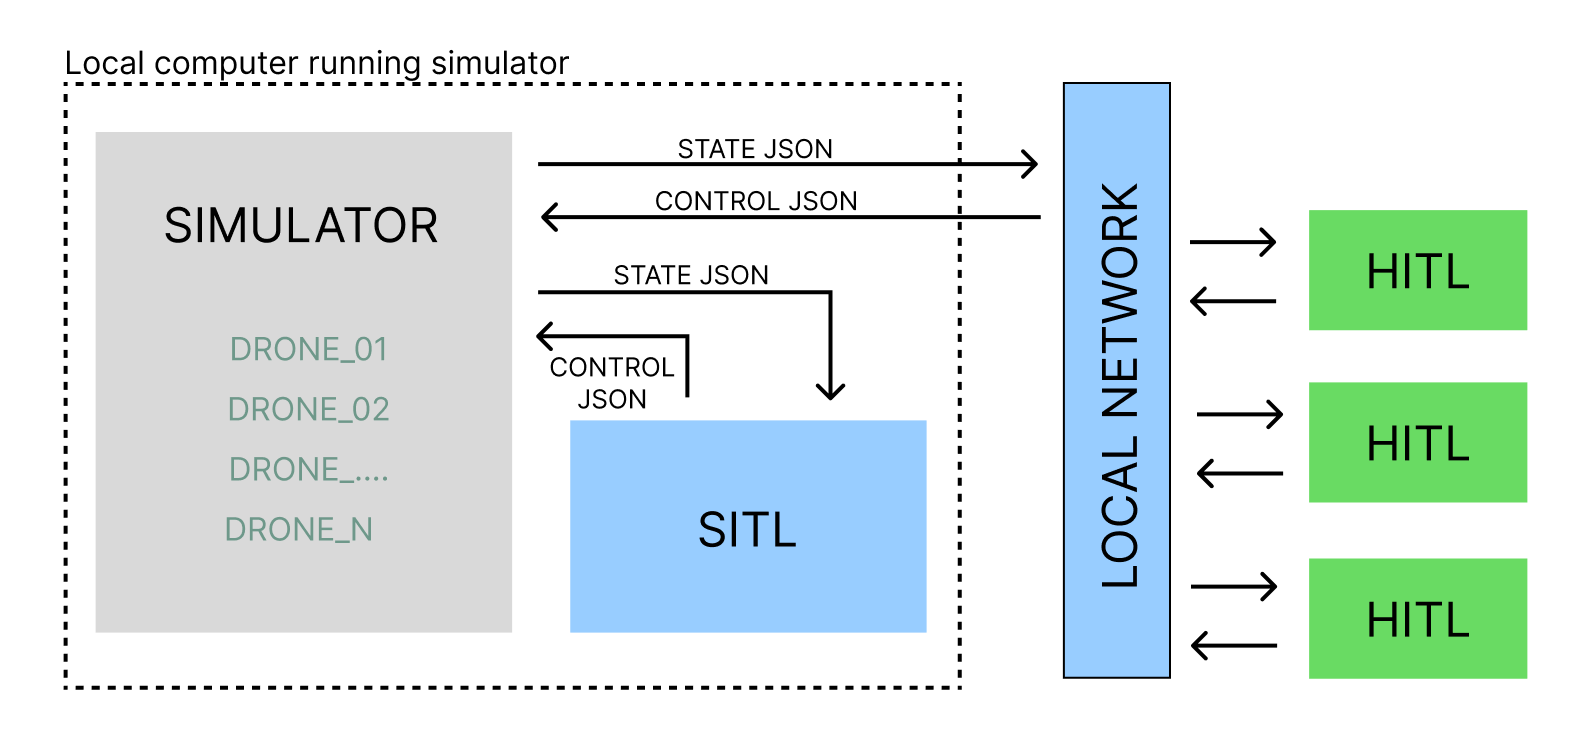
\includegraphics[width=0.8\textwidth]{images/SITL-HITL-diagram.png}
    \caption{Software-in-the-Loop and Hardware-in-the-Loop communication architecture.}
    \label{fig:sitl_hitl}
\end{figure}

 
 

 
% ── 3.5 SITL Mode ────────────────────────────────────────────────
\subsection{SITL Operation}
 
In SITL mode the controller executable runs on the same machine as simulator.
Each drone agent instance opens two UDP sockets on the loopback
interface and executes a fixed-rate control loop.
Upon receiving a state packet, the controller immediately computes and
transmits a command response, achieving a round-trip latency bounded by the
OS loopback stack (typically 1ms on Linux).
 
 
% ── 3.6 HITL Migration ───────────────────────────────────────────
\subsection{HITL Migration Path}
 
Transitioning from SITL to HITL requires modifications to only two files. 
The control logic, packet definitions, and configuration parameters remain identical across both modes.
 

\noindent The network topology changes from loopback to WiFi (IEEE 802.11),
introducing additional latency of approximately 5ms
on a local network. Given the low control bandwidth of surface vessels and the robustness of the communication protocol, this increase is well within acceptable limits for real-time control.
